\section{The \sysname Design} \label{sec:design}

We present the design of \sysname, a system that enhances existing DAG-based consensus protocols. We also argue the properties defined in \Cref{sec:goals}.

\subsection{DAG-based consensus protocols} \label{sec:dag}

Current DAG-based consensus protocols operate in logical \emph{rounds}. In each round, every honest (core) validator creates a unique signed vertex. Byzantine validators may attempt to equivocate by producing conflicting vertices or may abstain altogether. During each round, validators collect transactions from users and vertices from other validators to construct their next vertex. Each vertex must reference a minimum number of vertices from the previous round (typically $2f + 1$~\cite{narwhal,bullshark,mysticeti}) and adds fresh transactions that do not appear in preceding vertices.

\Cref{alg:core-validator} outlines the operations of core validators, aligning with nearly all existing structured DAG-based consensus protocols~\cite{narwhal,bullshark,shoal,shoal++,mysticeti,dag-rider,dumbo-ng,dispersedledger,sailfish,bbca-chain,fino,gradeddag,cordial-miners,wahoo,lightdag} and all DAG-based systems that have run in production~\cite{narwhal,bullshark,mysticeti,hammerhead}.

When a core validator receives a new vertex $v$, it invokes the function $\Call{ProcessCoreVertex}{v}$ (Line~\ref{alg:line:process-core-vertex}). The validator first downloads the causal history (Line~\ref{alg:line:sync-core-ancestors}) and verifies $v$ for validity (Line~\ref{alg:line:valid-core-vertex}), which typically involves checking signatures, validating parent vertex references, and ensuring syntactical correctness. A valid $v$ is then added to the local DAG view (Line~\ref{alg:line:add-to-dag}).

Next, the validator checks if the new vertex triggers any commits. It derives a set of \emph{leader} vertices either deterministically (in partially synchronous protocols~\cite{bullshark,shoal,mysticeti}) or by reconstructing a global perfect coin~\cite{abraham2023bingo} (in asynchronous protocols~\cite{narwhal,cordial-miners}). Using a protocol-specific decision rule, it analyzes DAG patterns to establish a total order among the leaders (Line~\ref{alg:line:commit-leaders}). If this yields a non-empty sequence, the validator linearizes the DAG into a sequence of vertices $C$ that it outputs to the application layer (Line~\ref{alg:line:linearize}). This linearization step uses a deterministic function like depth-first search over the sub-DAG defined by each leader in the sequence.

To advance the round, the validator attempts to create a new vertex $v'$ through $\Call{TryAdvance}{\;}$ (Line~\ref{alg:line:try-advance}). This succeeds if it possesses enough vertices from the previous round and, in partially synchronous protocols, enough leader vertices or if a timeout has occurred. If successful, the validator adds $v'$ to its local DAG view and broadcasts it to the other (core) validators (Line~\ref{alg:line:add-to-dag-2}). Creating a vertex may involve reliable or consistent broadcasting~\cite{dag-rider,narwhal,bullshark,shoal,shoal++}, a best-effort broadcast~\cite{mysticeti,cordial-miners}, or a hybrid of both~\cite{bbca-chain,gradeddag}.

\begin{algorithm}[t]
    \caption{Core Validator}
    \label{alg:core-validator}
    \algfontsize

    \begin{multicols}{2}
        \begin{algorithmic}[1]
            \State $T \gets \{ \; \}$ \Comment{Buffer client transactions}
            \State $\dag_c \gets \{ \; \}$ \Comment{DAG of core vertices}
            \change{\State $\dag_a \gets \{ \; \}$ \Comment{DAG of auxiliary vertices}}

            \Statex
            \Procedure{ProcessCoreVertex}{$v$} \label{alg:line:process-core-vertex}
            \State $\Call{SyncCoreAncestors}{v, \dag_c}$ \label{alg:line:sync-core-ancestors}
            \change{\State $\Call{SyncAuxAncestors}{v, \dag_a}$} \label{alg:line:sync-aux-ancestors}
            \State \require{$\Call{ValidCoreVertex}{v, \dag_c}$} \label{alg:line:valid-core-vertex}
            \State $\Call{AddToDag}{v, \dag_c}$ \label{alg:line:add-to-dag}
            \State $L \gets \Call{OrderNewLeaders}{\dag_c}$ \label{alg:line:commit-leaders}
            \If{$L \neq \perp $}
            \State $C \gets \Call{Linearize}{L, \dag_c, \change{\dag_a}}$ \label{alg:line:linearize}
            \State $\Call{OutputToApplication}{C}$
            \EndIf
            \State $\Call{TryAdvance}{\;}$
            \EndProcedure

            \Statex
            \Procedure{TryAdvance}{\;} \label{alg:line:try-advance}
            \State $v' \gets \Call{TryNewCoreVertex}{T, \dag_c, \change{\dag_a}}$ \label{alg:line:try-new-core-vertex}
            \If{$v' = \perp$} \Return \EndIf
            \State $\Call{AddToDag}{v', \dag_c}$ \label{alg:line:add-to-dag-2}
            \State $\Call{SendToCoreValidators}{v'}$ \label{alg:line:send-to-core-validators}
            \EndProcedure

            \Statex
            \change{
                \Procedure{ProcessAuxProposal}{$p$} \label{alg:line:process-aux-proposal}
                \State $\Call{SyncCoreAncestors}{v, \dag_c}$
                \State \require{$\Call{ValidAuxProposal}{v, \dag_c}$}
                \State $\sigma_p \gets \Call{Sign}{p}$
                \State $\Call{ReplyBack}{\sigma_p}$
                \EndProcedure
            }

            \Statex
            \change{
                \Procedure{ProcessAuxVertex}{$v$} \label{alg:line:process-aux-vertex}
                \State $\Call{DownloadCoreAncestors}{v, \dag_c}$
                \State \require{$\Call{ValidAuxVertex}{v, \dag_c}$}
                \State $\Call{AddToDag}{v, \dag_a}$
                \State $\Call{TryAdvance}{\;}$
                \EndProcedure
            }
        \end{algorithmic}
    \end{multicols}
\end{algorithm}
\begin{algorithm}[t]
    \caption{Auxiliary Validator}
    \label{alg:auxiliary-validator}
    \algfontsize

    \begin{algorithmic}[1]
        \State $T \gets \{ \; \}$ \Comment{Buffer client transactions}
        \State $\dag_c \gets \{ \; \}$ \Comment{DAG of core vertices}

        \Statex
        \Procedure{TryAdvance}{\;}
        \State $p \gets \Call{TryNewProposal}{T, \dag_c}$
        \If{$p = \perp$} \Return \EndIf
        \State $\{ \sigma_{(p,i)} \} \gets \Call{SendToCoreValidators}{p}$
        \State $v' \gets \Call{AssembleCertificate}{\{ \sigma_{(p,i)} \}}$
        \State $\Call{SendToCoreValidators}{v'}$
        \EndProcedure
    \end{algorithmic}
\end{algorithm}

\subsection{Block creation rule and commit rule} \label{sec:protocol}

We present the protocol for auxiliary validators and the modifications made to the core validator protocol, using \Cref{fig:dag} as an example. We denote vertices using the notation $v(author, round)$, where $author$ represents the validator that authored the vertex and $round$ indicates the round number.

\begin{figure}[t]
    \centering
    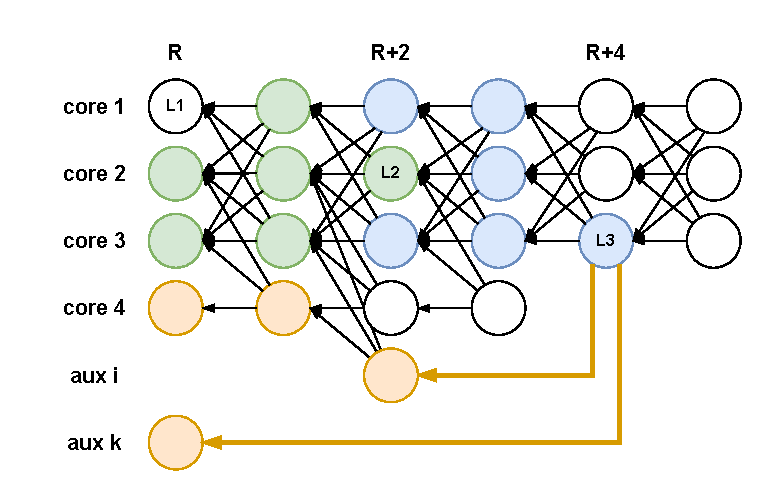
\includegraphics[width=0.8\textwidth]{figures/dag}
    \vskip -1em
    \caption{
        Example of \sysname execution with 4 core validators and $t_a = 2$.
    }
    \vskip -1em
    \label{fig:dag}
\end{figure}

\para{Auxiliary validators}
Auxiliary validators operate as full nodes, downloading the DAG generated by core validators while also collecting client transactions. \Cref{alg:auxiliary-validator} illustrates their protocol. Each auxiliary validator composes a signed \emph{proposal} containing client transactions and hash references to at least $2f + 1$ vertices created by core validators for a given round. They then send it to the core validators who check their validity and reply with a counter signature. The auxiliary validator then assembles a vertex, made up of the $2f + 1$ counter-signatures, and rebroadcasts it to all core validators. For example, $v_a(aux_i, R+2)$ references the vertices from round $R+1$ created by core validators $core_2$, $core_3$, and $core_4$. This protocol is essentially an instance of \emph{Byzantine consistent broadcast}~\cite{cachin2011introduction}driven by each individual auxiliary validator.
%
This design choice solves \textbf{challenge 1} by forgoing communication between auxiliary validators and leveraging the core validators as communication layer.

\para{Core validators}
\Cref{alg:core-validator} shows the modifications to the core validator's protocol in \change{orange}. Core validators execute $\Call{ProcessAuxProposal}{p}$ to validate, download the causal history, and counter-sign an auxiliary validator's proposal $p$. Since $p$ references $2f + 1$ core validator vertices, this verification allows core validators to synchronize any potentially missing vertices from the author of $p$. This protocol incentivizes auxiliary validators to collaborate, as inclusion of their vertices in the final commit sequence grants them a share of block rewards. The function $\Call{ProcessAuxVertices}{v_a}$ shows how core validators process a vertex $v_a$ (that is, a proposal $p$ counter-signed by $2f + 1$ core validators). Core validators add this vertex to a new map, $\dag_a$, which will later be merged into the DAG $\dag_c$ operated by core validators.
%
This design choice solves \textbf{challenge 2} by ensuring that malicious or unreliable auxiliary validators cannot affect the protocol once they delivered their vertex to a core validator. Since a correctly signed auxiliary vertex indicates that at least $2f + 1$ core validators possess its transaction data and causal history, the proposed data from auxiliary validators remains highly available despite their potential unreliability.

Next, we modify the vertex creation rules: every fixed number of rounds, the core validator leader (e.g., $L_3$ in \Cref{fig:dag}) must reference vertices from auxiliary validators with a joint stake totaling at least $t_a$ (see \Cref{sec:model}). In the figure, $L_3$ references $v_a(aux_i, R+2)$ and $v_a(aux_k, R)$.
%
This design solves \textbf{challenge 3} by allowing auxiliary validators to participate in the consensus without slowing it down. It essentially ensures that auxiliary validators can asynchronously create vertices at a slower pace than core validators without affecting the critical path of consensus, thus addressing challenge 3.

These auxiliary vertices are essentially treated as a \emph{weak link}~\cite{dag-rider} and core validators must first download them before processing $L_3$. Core validators do not use them to establish the order of the committed leaders but only during the linearization step of the DAG (Line~\ref{alg:line:linearize}). Designing \sysname to only operate at the linearization layer allows \sysname to generalize to most DAG-based protocols: the algorithm to order leader differs across protocols and thus \sysname leaves it untouched, but the linearization protocol is common to all these protocol.
In the example from \Cref{fig:dag}, assume the sequence of committed leaders (the output of \Cref{alg:line:commit-leaders}) is $[L_1, L_2, L_3]$. The validator linearizes the blocks within the sub-DAG defined by each leader block. If a block has already been linearized by a previous leader slot, the validator does not re-linearize it. The validator processes each leader sequentially, ensuring all blocks appear in the final commit sequence in a deterministic order according to their causal dependencies.

Auxiliary vertices are essentially treated as a \emph{weak link}~\cite{dag-rider}, with core validators required to download them before processing a vertex. Auxiliary vertices are not used to establish the order of committed leaders but are included during the linearization step (Line~\ref{alg:line:linearize}). Designing \sysname to operate only at the linearization layer makes it compatible with nearly all DAG-based protocols: while leader ordering algorithms vary across protocols, linearization is a common procedure. The validator linearizes the blocks within the sub-DAG defined by each leader block. If a block has already been linearized by a previous leader, the validator omits. Each leader is processed sequentially, ensuring all blocks appear in the final commit sequence in a deterministic order based on their causal dependencies.

In the example shown in \Cref{fig:dag}, the sequence of committed leaders (output from \Cref{alg:line:commit-leaders}) is ([$L_1$, $L_2$, $L_3$]).
$L_{1}$ does not define any sub-DAG (the process begins at round $R$), so only $L_1$ is added to the commit sequence.
$L_{2}$ defines a sub-DAG of the green blocks, which are linearly ordered, as e.g., $v_c(core_1,R+1)$, $v_c(core_2,R)$, $v_c(core3,R)$, $v_c(core_2,R+1)$, $v_c(core_3,R+1)$, and $L_2$.
While processing $L_3$, which defines a sub-DAG of both blue and orange vertices, the validator collects and linearizes all such vertices. As a result, although the original DAG might exclude the core orange vertices ($v_c(core_4, R)$ and $v_c(core_4, R+1)$) and may omit the auxiliary vertices ($v_a(aux_i,R+2)$ and $v_a(aux_k,R)$), \sysname guarantees their inclusion in the final commit sequence. This inclusion helps core validator $core_3$ to synchronize parts of the DAG that were potential missing from its local view.

\subsection{Security analysis} \label{sec:security}
\alberto{Mention a simple safety and liveness argument.}
